\documentclass[border=3pt]{standalone}
\usepackage[T1]{fontenc}
\usepackage[utf8]{inputenc}
\usepackage{lmodern}
\usepackage{amsmath,amssymb}
\usepackage{xcolor}
\usepackage{tikz}
\usepackage{fontawesome5}
\usepackage{ragged2e}
\usetikzlibrary{shapes,shapes.geometric,shapes.misc,arrows.meta,positioning,
                calc,fit,backgrounds,decorations.pathreplacing,
                decorations.markings,patterns,chains}
\usetikzlibrary{decorations.pathreplacing,decorations.markings}
\definecolor{primary}{HTML}{1A5276}
\definecolor{secondary}{HTML}{2E86C1}
\definecolor{accent}{HTML}{E74C3C}
\definecolor{lightbg}{HTML}{EBF5FB}
\definecolor{defbg}{HTML}{FDF2E9}
\definecolor{greenhl}{HTML}{27AE60}
\definecolor{purplehl}{HTML}{8E44AD}
\definecolor{goldhl}{HTML}{B7950B}
\definecolor{tealhl}{HTML}{117A65}
\definecolor{codebg}{HTML}{F4F6F7}
\definecolor{neutral}{HTML}{707B7C}
\definecolor{dom1}{HTML}{1F618D}
\definecolor{dom2}{HTML}{117864}
\definecolor{dom3}{HTML}{6C3483}
\definecolor{dom4}{HTML}{922B21}
\definecolor{dom5}{HTML}{B7950B}
% --- carried over from ccna.sty so figures match the book exactly
\tikzset{
  dev/.style={rounded corners=3pt, draw=#1, fill=#1!8, text=#1!45!black,
              line width=0.9pt, minimum width=1.45cm, minimum height=1.05cm,
              align=center, font=\scriptsize\bfseries, inner sep=2pt},
  wirestyle/.style={line width=0.9pt, neutral!75},
  xconn/.style={line width=0.9pt, neutral!75, dash pattern=on 2.5pt off 2pt},
}

\newcommand{\Rtr}[3]{\node[dev=dom3] (#1) at #2 {\faIcon{route}\\#3};}
\newcommand{\Sw}[3]{\node[dev=dom2] (#1) at #2 {\faIcon{sitemap}\\#3};}
\newcommand{\Msw}[3]{\node[dev=dom3] (#1) at #2 {\faIcon{layer-group}\\#3};}
\newcommand{\Host}[3]{\node[dev=neutral] (#1) at #2 {\faIcon{desktop}\\#3};}
\newcommand{\Lap}[3]{\node[dev=neutral] (#1) at #2 {\faIcon{laptop}\\#3};}
\newcommand{\Srv}[3]{\node[dev=dom1] (#1) at #2 {\faIcon{server}\\#3};}
\newcommand{\Ap}[3]{\node[dev=dom5] (#1) at #2 {\faIcon{wifi}\\#3};}
\newcommand{\Wlc}[3]{\node[dev=dom5] (#1) at #2 {\faIcon{broadcast-tower}\\#3};}
\newcommand{\Fw}[3]{\node[dev=dom4] (#1) at #2 {\faIcon{shield-alt}\\#3};}
\newcommand{\Cld}[3]{\node[dev=neutral] (#1) at #2 {\faIcon{cloud}\\#3};}
\newcommand{\Phone}[3]{\node[dev=dom5] (#1) at #2 {\faIcon{phone-alt}\\#3};}
\newcommand{\Prn}[3]{\node[dev=neutral] (#1) at #2 {\faIcon{print}\\#3};}

% A link. The optional argument takes tikz options (e.g. xconn for a
% trunk drawn dashed); the fourth argument labels the link.
\newcommand{\wire}[4][wirestyle]{%
  \draw[#1] (#2) -- node[font=\tiny, text=neutral!85!black, fill=white,
                          inner sep=1.2pt, midway] {#4} (#3);}
\newcommand{\plainwire}[3][wirestyle]{\draw[#1] (#2) -- (#3);}


\newenvironment{topology}[1][]
  {\begin{center}\begin{tikzpicture}[font=\scriptsize,#1]}
  {\end{tikzpicture}\end{center}}


\newcommand{\cmd}[1]{\texttt{\small #1}}
\newcommand{\term}[1]{\textbf{\textcolor{primary}{#1}}}
\newcommand{\chref}[1]{Chapter~\ref{ch:#1}}
\newcommand{\ccnafitw}[1]{#1}
\providecommand{\thefigure}{}
% --- progressive builds
\newcount\buildlevel \buildlevel=99
\newcommand{\stepvis}[2]{\ifnum#1>\buildlevel\relax\else#2\fi}
\begin{document}
\begin{tikzpicture}[font=\scriptsize]
  \tikzset{
    dv/.style={rounded corners=3pt, draw=#1, fill=#1!8, text=#1!45!black,
               line width=0.9pt, minimum width=1.25cm, minimum height=0.9cm,
               align=center, font=\tiny\bfseries},
    w/.style={line width=0.8pt, neutral!60},
    fl/.style={-{Stealth[length=2.2mm]}, line width=1.1pt},
    hdr/.style={font=\scriptsize\bfseries, text=neutral!45!black}}

  %================ panel 1: unknown destination -> flood
  \node[hdr] at (3.0,2.9) {1. Destination unknown $\rightarrow$ \textcolor{accent!80!black}{flood}};
  \node[dv=dom2, minimum width=4.6cm] (s1) at (3.0,1.35) {\faIcon{sitemap}\\SW1};
  \foreach \x/\n in {1.1/A, 2.35/B, 3.65/C, 4.9/D}
    \node[dv=neutral] at (\x,-0.35) {\faIcon{desktop}\\PC-\n};
  \draw[fl, dom2!80] (1.1,0.1) -- (1.1,0.9);
  \foreach \x in {2.35, 3.65, 4.9} \draw[fl, accent!75] (\x,0.9) -- (\x,0.1);
  \node[font=\tiny, text=dom2!45!black, anchor=east] at (0.85,0.5) {in};
  \node[font=\tiny, text=neutral!85!black, align=center] at (3.0,-1.3)
      {the frame goes everywhere except\\back out of the port it arrived on};

  %================ panel 2: learned -> forward
  \node[hdr] at (11.0,2.9) {2. Now learned $\rightarrow$ \textcolor{dom2!70!black}{forward}};
  \node[dv=dom2, minimum width=4.6cm] (s2) at (11.0,1.35) {\faIcon{sitemap}\\SW1};
  \foreach \x/\n in {9.1/A, 10.35/B, 11.65/C, 12.9/D}
    \node[dv=neutral] at (\x,-0.35) {\faIcon{desktop}\\PC-\n};
  \draw[fl, dom2!80] (12.9,0.1) -- (12.9,0.9);
  \draw[fl, dom2!80] (9.1,0.9) -- (9.1,0.1);
  \node[font=\tiny, text=neutral!85!black, align=center] at (11.0,-1.3)
      {PC-D replied, so the table now holds it.\\One port, not three};

  %================ the table between them
  \node[draw=neutral!55, fill=codebg, rounded corners=2pt, line width=0.7pt,
        font=\tiny\ttfamily, align=left, inner sep=4pt] at (7.05,1.2)
      {MAC address table\\[2pt]
       \textcolor{neutral!70!black}{aaaa.aaaa.aaaa~~Gi0/1}\\
       \textcolor{accent!70!black}{dddd.dddd.dddd~~Gi0/4}};
  \node[font=\tiny, text=accent!70!black, align=center] at (7.05,0.05)
      {learned from\\the reply};
\end{tikzpicture}
\end{document}
